\documentclass[11pt,a4paper]{article}
\usepackage[margin=2.2cm]{geometry}
\usepackage{graphicx}
\usepackage{booktabs}
\usepackage{float}
\usepackage{amsmath}
\usepackage{xcolor}
\usepackage{microtype}
\usepackage{fancyvrb}
\usepackage[colorlinks=true,linkcolor=blue!50!black,urlcolor=blue!60!black]{hyperref}
\makeatletter\g@addto@macro{\UrlBreaks}{\UrlOrds}\makeatother % allow long URLs to wrap
\setlength{\parskip}{0.5em}
\setlength{\parindent}{0pt}

\newcommand{\repo}{\url{https://github.com/gb0x11/CS6886W-Assignment-2}}
\newcommand{\BaselineAcc}{95.36}
\newcommand{\BaselineTrainAcc}{99.93}
\newcommand{\BaselineEpochs}{200}
\newcommand{\BaselineBestEpochAcc}{95.39}
\newcommand{\BaselineHours}{5.0}
\newcommand{\FPModelMB}{8.663}
\newcommand{\FPModelBytes}{9,083,592}
\newcommand{\BestName}{final\_mix2.5\_a5\_f8\_l8\_al6\_e40}
\newcommand{\BestAcc}{94.48}
\newcommand{\BestDrop}{0.88}
\newcommand{\BestSizeMB}{0.719}
\newcommand{\BestSizeBytes}{753,672}
\newcommand{\BestRatio}{12.05}
\newcommand{\BestWeightRatio}{12.88}
\newcommand{\BestActRatio}{6.24}
\newcommand{\BestActPeakRatio}{6.30}
\newcommand{\BestAvgWBits}{2.48}
\newcommand{\BestAvgABits}{5.13}
\newcommand{\BestOverheadPct}{9.2}
\newcommand{\BestOverheadBytes}{69,640}
\newcommand{\BestActMB}{1.048}
\newcommand{\FPActMB}{6.542}
\newcommand{\BestActPeakMB}{0.193}
\newcommand{\FPActPeakMB}{1.219}
\newcommand{\BestActMeasuredBytes}{1,099,240}
\newcommand{\BestFakeQuantAcc}{94.55}
\newcommand{\BestPtqAcc}{93.48}
\newcommand{\BestEpochs}{40}
\newcommand{\NumRuns}{21}
\newcommand{\MaxRatio}{14.41}
\newcommand{\MaxWeightRatio}{15.71}
\newcommand{\MaxActRatio}{10.63}
\newcommand{\BestABits}{5}
\newcommand{\BestALinBits}{6}
\newcommand{\LinActPct}{12}
\newcommand{\SmallWeightPct}{0.6}
\newcommand{\BestWeightBytes}{684,032}
\newcommand{\FPWeightBytes}{8,810,240}
\newcommand{\BestMinWBits}{2}
\newcommand{\BestMaxWBits}{8}
\newcommand{\BestTwoBitLayers}{17}
\newcommand{\BestActFPHookBytes}{6,859,816}
\newcommand{\BestTrainMin}{104}
\newcommand{\BestCkptMB}{0.770}
\newcommand{\BestLr}{0.004}

\newcommand{\wbprojecturl}{https://forge.coreweave.com/wandb/cs25m508-indian-institute-of-technology/cs6886w-a2-mobilenetv2-compression}
\newcommand{\wbreporturl}{https://forge.coreweave.com/wandb/cs25m508-indian-institute-of-technology/cs6886w-a2-mobilenetv2-compression/reports/CS6886W-A2:-MobileNet-v2-compression-sweep--VmlldzoxODMwNDQ3NA==}
\newcommand{\wblinks}{\href{\wbprojecturl}{W\&B project (all runs)}\quad\textbullet\quad\href{\wbreporturl}{W\&B report with the parallel-coordinates chart}}


\begin{document}

\begin{center}
{\LARGE\bfseries CS6886W: Systems Engineering for Deep Learning}\\[4pt]
{\Large Assignment 2: Compressing MobileNet-v2 on CIFAR-10}\\[10pt]
{\large Gowtham B \quad (CS25M508)}\\[6pt]
GitHub repository: \repo\\
\wblinks
\end{center}

\section*{Summary of the required results}

\begin{center}
\begin{tabular}{p{0.52\linewidth}p{0.42\linewidth}}
\toprule
Required item & Result \\
\midrule
Accuracy of the model without any compression & \textbf{\BaselineAcc\%} test top-1 (FP32 MobileNet-v2) \\
Accuracy of the final compressed model & \textbf{\BestAcc\%} test top-1 (drop of \BestDrop{} points) \\
Storage overheads (scales, biases, metadata) & \BestOverheadBytes{} bytes, \BestOverheadPct\% of the compressed model (Question 2c) \\
Best compression ratio of the model (in memory) & \textbf{\BestRatio$\times$} (\FPModelMB{} MB $\to$ \BestSizeMB{} MB) \\
Best compression ratio of the weights (in memory) & \textbf{\BestWeightRatio$\times$} (\BestAvgWBits{} bits per weight on average) \\
Best compression ratio of the activations & \textbf{\BestActRatio$\times$} over all feature maps of one image, \BestActPeakRatio$\times$ at the memory peak (measured as described in Question 4b) \\
W\&B parallel-coordinates chart & Figure~\ref{fig:parallel} (\NumRuns{} compression runs) \\
Final approximated model size after compression & \textbf{\BestSizeMB{} MB} (\BestSizeBytes{} bytes) \\
\bottomrule
\end{tabular}
\end{center}

All ratios refer to one and the same model, \texttt{\BestName}, the final model of this report. ``MB'' means $2^{20}$ bytes, as in the course template. Every size is an in-memory size: the compressed model is held in RAM as bit-packed integer codes and it runs inference from that form. No compression library or API is used; the quantizers, the bit-packing and the size accounting are written from scratch (\texttt{compressor/} in the repository).

%=====================================================================
\section*{Question 1: Training baseline}

\subsection*{(a) Data preparation and transforms}

CIFAR-10 has 50{,}000 training and 10{,}000 test images of $32\times32$ pixels. The network is trained on all 50{,}000 training images; the test set is used only to report accuracy. No early stopping and no checkpoint selection is done on the test set: the reported model is the one after the last epoch.

\begin{center}
\small
\begin{tabular}{lll}
\toprule
Split & Transform (in order) & Parameters \\
\midrule
Train & RandomCrop & $32\times32$ crop after zero-padding 4 px per side \\
      & RandomHorizontalFlip & $p=0.5$ \\
      & ToTensor & uint8 $[0,255]\to$ float $[0,1]$ \\
      & Normalize & mean $(0.4914, 0.4822, 0.4465)$, std $(0.2470, 0.2435, 0.2616)$ \\
      & Cutout & one $16\times16$ square set to 0 (the mean after normalization) \\
\midrule
Test & ToTensor, Normalize & same mean and std, no augmentation \\
\bottomrule
\end{tabular}
\end{center}

The mean and standard deviation are the per-channel statistics of the CIFAR-10 training pixels, so the inputs have zero mean and unit variance. Random crops and flips encode the translation and mirror invariance of natural images; Cutout hides a random quarter of the image and forces the network to use several parts of the object. To avoid a data-loading bottleneck on a laptop GPU, the dataset is kept on the GPU as uint8 tensors and the transforms are applied there per mini-batch (\texttt{mbv2/data.py}), with random numbers drawn from a seeded generator.

\subsection*{(b) MobileNet-v2 configuration and training strategy}

\textbf{Architecture} (\texttt{mbv2/model.py}, written from scratch after the torchvision layout). MobileNet-v2 is a stack of inverted residual blocks: a $1\times1$ convolution expands the channels by a factor $t$, a $3\times3$ depthwise convolution filters them, and a $1\times1$ convolution projects back to a narrow ``linear bottleneck'' without a non-linearity. Blocks that keep resolution and width have a residual connection.

\begin{center}
\small
\begin{tabular}{llrrrr}
\toprule
Stage & Operator & Expansion $t$ & Output channels & Repeats & Stride \\
\midrule
Stem & $3\times3$ conv, BN, ReLU6 & & 32 & 1 & 1 \\
1 & inverted residual & 1 & 16 & 1 & 1 \\
2 & inverted residual & 6 & 24 & 2 & 1 \\
3 & inverted residual & 6 & 32 & 3 & 2 \\
4 & inverted residual & 6 & 64 & 4 & 2 \\
5 & inverted residual & 6 & 96 & 3 & 1 \\
6 & inverted residual & 6 & 160 & 3 & 2 \\
7 & inverted residual & 6 & 320 & 1 & 1 \\
Head & $1\times1$ conv, BN, ReLU6 & & 1280 & 1 & 1 \\
     & global average pool, dropout, linear & & 10 & 1 & \\
\bottomrule
\end{tabular}
\end{center}

\begin{itemize}
\item \textbf{Width multiplier} 1.0 (the standard network): 2{,}236{,}682 parameters, of which 2{,}202{,}560 are convolution or linear weights in 53 layers (52 convolutions and the classifier).
\item \textbf{CIFAR adaptation.} The ImageNet network downsamples by 32, which would reduce a $32\times32$ image to a single pixel. The stem and stage 2 therefore use stride 1 instead of 2 (the usual CIFAR variant), so the network downsamples by 8 and the last feature map is $4\times4$. Nothing else is changed.
\item \textbf{BatchNorm} after every convolution (52 layers), default settings (momentum 0.1, $\epsilon=10^{-5}$), scale initialised to 1 and shift to 0. \textbf{ReLU6} activations, none after the projection convolutions.
\item \textbf{Dropout} 0.2 before the classifier (the torchvision default). Convolutions are initialised with the Kaiming normal scheme (fan-out), the classifier with $\mathcal N(0, 0.01^2)$.
\end{itemize}

\textbf{Training strategy} (\texttt{train.py}).
\begin{center}
\small
\begin{tabular}{ll}
\toprule
Setting & Value \\
\midrule
Optimizer & SGD with Nesterov momentum 0.9 \\
Learning rate & peak 0.1; linear warm-up over 5 epochs, then cosine decay to 0 (per step) \\
Epochs / batch size & \BaselineEpochs{} / 128 (390 steps per epoch, last partial batch dropped) \\
Weight decay & $5\times10^{-4}$ on convolution and linear weights only (not on BatchNorm or biases) \\
Label smoothing & 0.1 \\
Other regularization & dropout 0.2, crop + flip + Cutout(16) \\
Seed & 42 (Python, NumPy, PyTorch, shuffling, augmentation) \\
Hardware & Apple M1 Pro (16 GB), PyTorch 2.14.1 MPS backend, about 90 s per epoch \\
\bottomrule
\end{tabular}
\end{center}

SGD with Nesterov momentum and a cosine schedule is the standard recipe for CIFAR networks; the warm-up avoids instabilities of the randomly initialised BatchNorm network at learning rate 0.1. Weight decay is not applied to BatchNorm parameters and biases because shrinking them does not regularize the function and hurts small depthwise networks. Label smoothing and Cutout counter over-fitting in a long schedule.

\subsection*{(c) Final test accuracy, curves and failure modes}

\BaselineText

%=====================================================================
\section*{Question 2: Model compression implementation}

\subsection*{(a) The compression method and its design choices}

The method combines five parts, all implemented in \texttt{compressor/} without any library quantization, pruning or packing function.

\textbf{1. Uniform quantization with a learned step} (\texttt{quantizers.py}). A $b$-bit quantizer stores an integer code per value and reconstructs a multiple of a step $s$:
\[
\text{code} = \mathrm{clamp}\!\left(\mathrm{round}(x/s),\, q_n,\, q_p\right), \qquad \hat x = s\cdot\text{code},
\]
with $(q_n, q_p) = (-2^{b-1},\, 2^{b-1}-1)$ for signed tensors and $(0,\, 2^b-1)$ for unsigned ones. The step is first set by a search that minimises the squared quantization error $\lVert x-\hat x\rVert^2$ over 60 clipping thresholds (this clips rare outliers instead of wasting levels on them, which is what makes low bit-widths usable) and is then trained together with the weights, as in Learned Step Size Quantization (LSQ). The rounding uses the straight-through estimator. The backward pass is written by hand,
\[
\frac{\partial \hat x}{\partial x} = \mathbf 1[q_n \le x/s \le q_p], \qquad
\frac{\partial \hat x}{\partial s} = \begin{cases}\mathrm{round}(x/s) - x/s & q_n \le x/s \le q_p\\ q_n \text{ or } q_p & \text{otherwise,}\end{cases}
\]
with the step gradient scaled by $1/\sqrt{N q_p}$; it stores two small tensors per quantizer instead of the five or six of an equivalent chain of autograd operations, which matters on a 16 GB machine.

\textbf{2. Weights: signed, one step per output channel.} The channels of a depthwise convolution differ in range by orders of magnitude, so a single step per layer (as in the course template) destroys MobileNets below 8 bits. Each output channel therefore has its own step. This costs one number per channel, which the BatchNorm folding below makes free.

\textbf{3. Activations: every tensor that is kept in memory between two layers is quantized.} Outputs of ReLU6 layers are non-negative and use unsigned codes, with the clipping range learned (it starts at or below 6). The outputs of the linear projection convolutions and the residual sums take both signs and use signed codes. The input image is not quantized further: CIFAR-10 pixels are 8-bit integers, so the normalised input is exactly representable by its uint8 codes, and the compressed model takes raw uint8 images. The 10 logits stay in full precision.

\textbf{4. Configurable, mixed precision} (\texttt{config.py}, \texttt{sensitivity.py}). The bit-width is a parameter of every tensor. The command line exposes a global weight and activation bit-width (the template's \texttt{--weight\_quant\_bits} and \texttt{--activation\_quant\_bits}), separate bit-widths for the stem, the depthwise layers, the classifier and the linear activations, and a per-layer table. That table can be produced automatically by a \emph{sensitivity-guided allocator}: for every layer and every candidate bit-width (2, 3, 4, 5, 6, 8) it quantizes only that layer and measures the KL divergence between the full-precision and the perturbed predictions on 2{,}000 training images; then, starting from 8 bits everywhere, it repeatedly lowers the bit-width of the layer where this costs the least divergence per bit of memory saved, until a requested average bit-width is reached. Layers differ in size by a factor of 470 (864 weights in the stem, 409{,}600 in the head), so the same bit-width everywhere wastes memory: large redundant layers can go to 2 bits while small sensitive ones keep 6 to 8.

\textbf{5. Accuracy recovery by quantization-aware fine-tuning with distillation} (\texttt{compress.py}). After calibration (which is already post-training quantization, PTQ), the quantized network is fine-tuned for a few epochs with quantization in the forward pass (QAT). The loss is $0.3\,\mathrm{CE}(y) + 0.7\,T^2\,\mathrm{KL}(\text{teacher}\,\Vert\,\text{student})$ with temperature $T=4$, where the teacher is the full-precision baseline: the compressed network is asked to reproduce the function it replaces. SGD with Nesterov momentum, learning rate 0.01 with cosine decay, weight decay $10^{-4}$, no dropout, the same augmentation as the baseline.

\textbf{The in-memory format} (\texttt{packing.py}, \texttt{packed.py}). The final model is exported to a \texttt{PackedMobileNetV2}: the integer weight codes of every layer are bit-packed into a byte buffer, so $n$ codes of $b$ bits occupy exactly $\lceil nb/8\rceil$ bytes for any $b$ from 1 to 16 (two 4-bit weights per byte, eight 3-bit weights in three bytes). This is fixed-width packing with shifts and masks, not entropy coding: any weight can be read at a fixed offset, and the buffer is the form in which the model sits in RAM, not just a smaller file. The packed model runs inference directly from this state. PyTorch has no convolution kernels for sub-byte integers, so each layer's codes are expanded to a temporary float tensor while that layer executes and released afterwards; what persists is only the packed state. All accuracies of compressed models in this report are measured on the packed model itself.

\textbf{Why these choices.} (i) Quantization, unlike unstructured pruning or weight clustering, reduces the size of weights \emph{and} activations with one mechanism and maps to integer hardware. (ii) Per-channel steps and learned clipping address the two known weaknesses of MobileNets under quantization: uneven depthwise channel ranges and the narrow linear bottlenecks. (iii) Mixed precision spends bits where they matter. (iv) Distillation uses the baseline as a free, noise-free target. (v) Everything that is not a weight code is counted explicitly (Question 2c), so the reported ratios are not optimistic.

\subsection*{(b) How the compression is applied to MobileNet-v2}

\textbf{All 53 weight layers are compressed}; there is no layer left in FP32. Table~\ref{tab:layers} gives the bit-widths of the final model by layer type and Figure~\ref{fig:bits} per layer.

\begin{table}[H]
\centering
\small
\begin{tabular}{lrrlrrl}
\toprule
Layer type & Layers & Weights & Weight bits & Code bytes & Overhead bytes & Output activation \\
\midrule
Stem 3x3 conv & 1 & 864 & 8 & 864 & 152 & 5-bit unsigned \\
1x1 expand convs & 16 & 751,872 & 2 to 5 & 196,848 & 28,800 & 5-bit unsigned \\
3x3 depthwise convs & 17 & 64,224 & 3 to 8 & 28,368 & 28,952 & 5-bit unsigned \\
1x1 project convs (linear) & 17 & 963,200 & 2 to 6 & 291,552 & 6,424 & 6-bit signed \\
Head 1x1 conv & 1 & 409,600 & 3 & 153,600 & 5,144 & 5-bit unsigned \\
Classifier (linear) & 1 & 12,800 & 8 & 12,800 & 56 & logits, FP32 \\
\midrule
Total & 53 & 2,202,560 & 2.48 (avg) & 684,032 & 69,528 & \\
\bottomrule
\end{tabular}

\caption{Compression of the final model \texttt{\BestName} by layer type. Overhead bytes are the per-channel scales and biases and 16 bytes of metadata per layer.}
\label{tab:layers}
\end{table}

\begin{figure}[H]
\centering
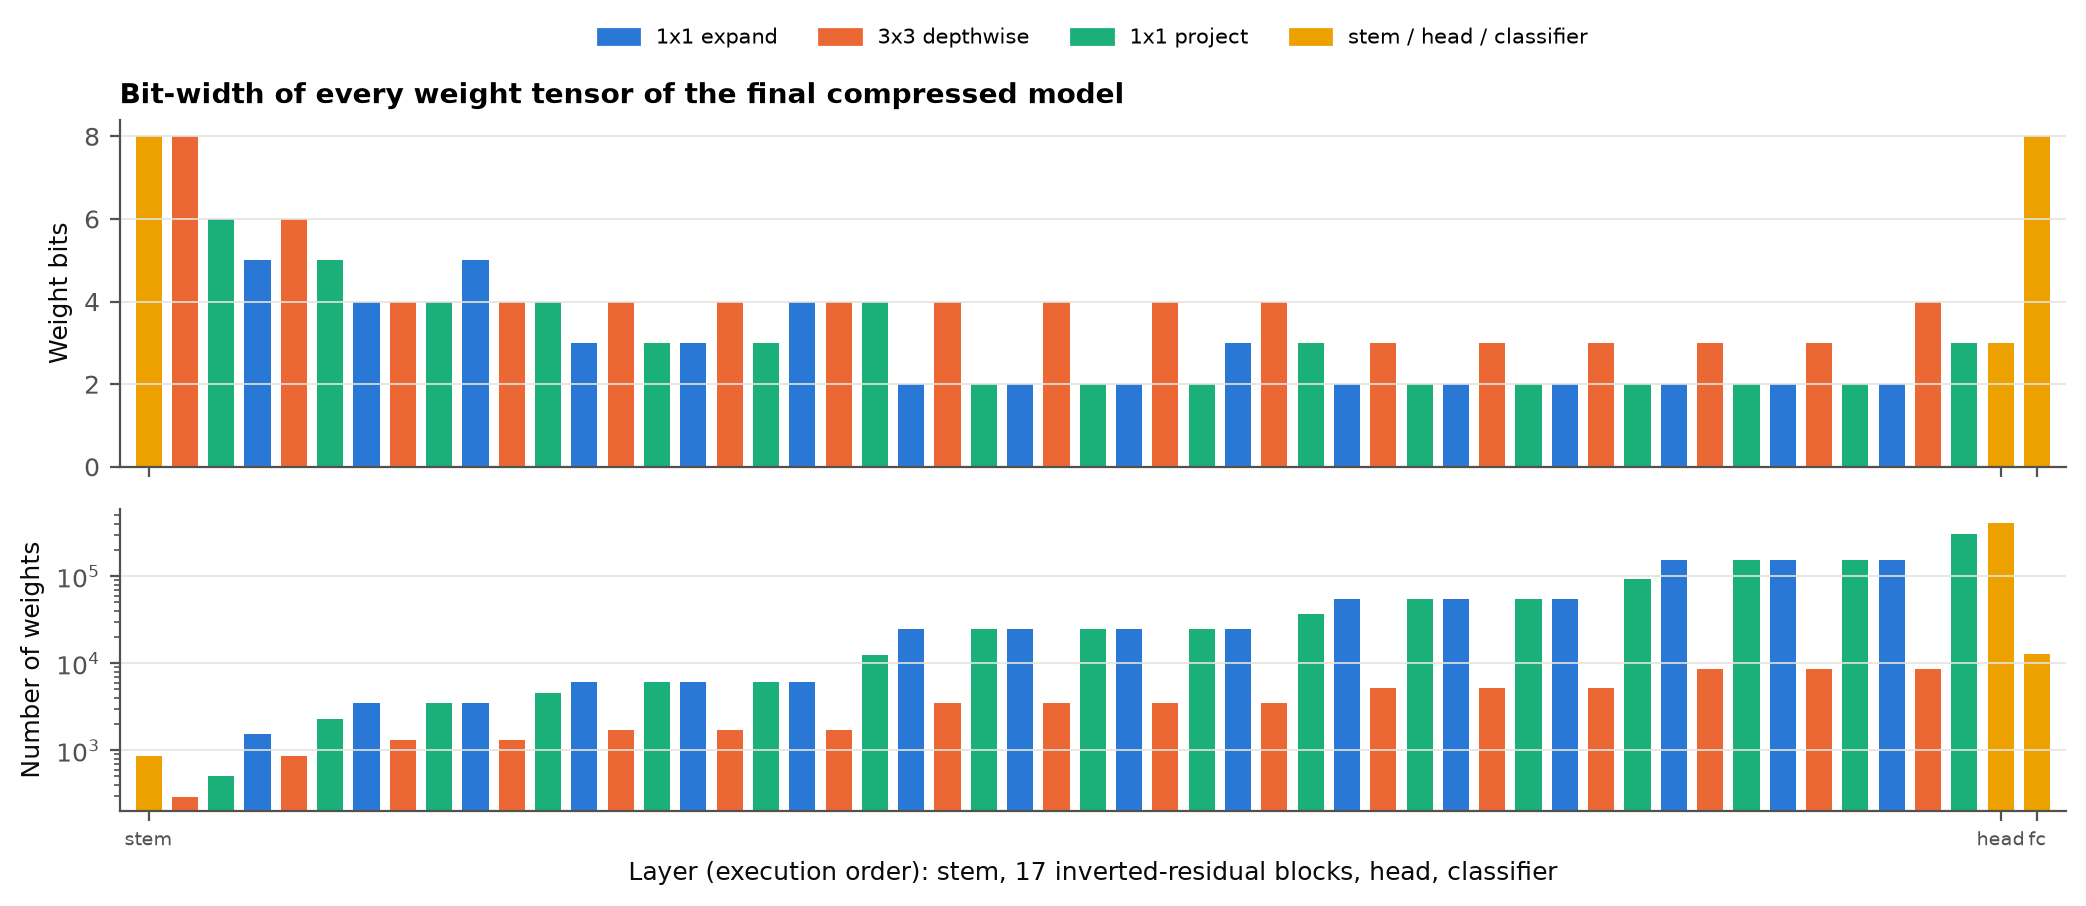
\includegraphics[width=\linewidth]{figures/bit_allocation.png}
\caption{Bit-width (top) and size (bottom, log scale) of the 53 weight tensors of the final model.}
\label{fig:bits}
\end{figure}

\IfFileExists{figures/sensitivity.png}{%
\begin{figure}[H]
\centering
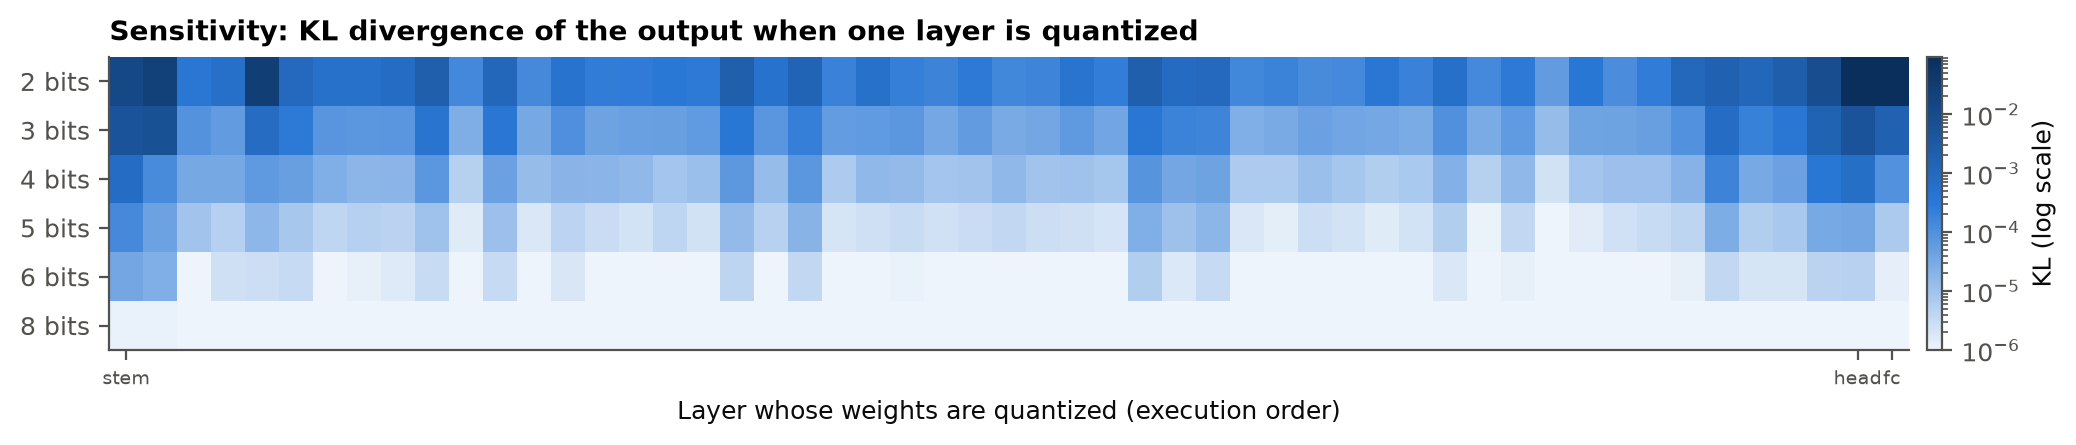
\includegraphics[width=\linewidth]{figures/sensitivity.png}
\caption{Measured sensitivity of every layer to weight quantization, the input of the bit allocator.}
\label{fig:sens}
\end{figure}}{}

\textbf{BatchNorm is folded away.} During fine-tuning each convolution is followed by its BatchNorm, which keeps training stable. At export, with weights $W = s_c\cdot\text{code}$ ($s_c$ the learned step of output channel $c$),
\[
\mathrm{BN}(\mathrm{conv}(x, W))_c = \mathrm{conv}(x, \text{code})_c \cdot \underbrace{\frac{s_c\,\gamma_c}{\sqrt{\sigma_c^2+\epsilon}}}_{\text{scale}_c} \;+\; \underbrace{\beta_c - \frac{\mu_c\,\gamma_c}{\sqrt{\sigma_c^2+\epsilon}}}_{\text{bias}_c},
\]
so the four BatchNorm vectors and the quantizer step collapse into one scale and one bias per channel, and the integer codes are exactly the ones that were trained. All 52 BatchNorm layers disappear from the compressed model.

\textbf{Exceptions and special cases.}
\begin{itemize}
\item \emph{Input image:} kept as its native 8-bit pixels (lossless), not reduced to the activation bit-width.
\item \emph{Logits:} the 10 outputs stay in FP32 (40 bytes).
\item \emph{Sensitive, tiny tensors:} in the final model the stem (864 weights) and the classifier (12{,}800 weights) keep 8-bit weights, and the linear-bottleneck outputs, residual sums and the pooled feature vector keep 8-bit activations. These tensors are 12\% of the activation memory and 0.6\% of the weights, and the network is most sensitive to them (Question 3).
\item \emph{Scales and biases} are stored in FP16 rather than quantized to a few bits.
\item \emph{Residual connections:} the sum of a block input and the block output is a new stored tensor and gets its own quantizer.
\item \emph{Dropout} is an identity at inference and has no parameters.
\end{itemize}

\subsection*{(c) Storage overheads}

Besides the weight codes, the compressed model has to keep the following in memory. All of it is included in every model size and model compression ratio of this report.

\begin{table}[H]
\centering
\small
\begin{tabular}{lllrr}
\toprule
Component & Count & Precision & Bytes & Share (\%) \\
\midrule
Weight codes (bit-packed) & 2,202,560 weights & 2.48 bits (avg) & 684,032 & 90.76 \\
Per-channel scales & 17,066 channels & 16 bits (FP16) & 34,132 & 4.53 \\
Per-channel biases & 17,066 channels & 16 bits (FP16) & 34,132 & 4.53 \\
Activation quantizer steps & 63 quantizers & 8 bytes each & 504 & 0.07 \\
Layer metadata, input mean / std & 53 layers & 16 bytes each + 24 & 872 & 0.12 \\
\midrule
Compressed model & & & 753,672 & 100.00 \\
of which overhead & & & 69,640 & 9.24 \\
FP32 model (parameters + BatchNorm buffers) & & 32 bits & 9,083,592 & \\
\bottomrule
\end{tabular}

\caption{In-memory size of the final model \texttt{\BestName}, split into weight codes and overheads.}
\label{tab:overheads}
\end{table}

\begin{itemize}
\item \textbf{Per-channel scale and bias}: one FP16 number each for the 17{,}056 convolution output channels and the 10 classifier outputs. This is the dominant overhead. It replaces the four FP32 BatchNorm vectors per channel of the baseline (which are counted in the FP32 model size, since they are needed at inference).
\item \textbf{Activation quantizer parameters}: one FP32 step plus bit-width and sign per quantizer, counted as 8 bytes each.
\item \textbf{Layer metadata}: bit-width, sign and tensor shape, counted as 16 bytes per layer, and the input mean and standard deviation (24 bytes).
\item \textbf{Byte padding}: each layer is packed separately, so each one is rounded up to a whole byte (at most 53 bytes in total; included in the weight-code bytes).
\end{itemize}
The sizes are obtained by adding up the bytes of the actual buffers of the packed model (\texttt{PackedMobileNetV2.size\_report}); unit tests check them against hand counts. The FP32 reference is measured the same way from the tensors of the uncompressed model: 2{,}236{,}682 parameters and 34{,}164 BatchNorm buffer values, \FPModelBytes{} bytes.

%=====================================================================
\section*{Question 3: Compression results}

\subsection*{(a) Compression at different levels}

\SweepIntro

\begin{table}[H]
\centering
\footnotesize
\begin{tabular}{llrrrrrrrr}
\toprule
Run & Method & \shortstack{W bits\\(avg)} & \shortstack{A bits\\(ReLU6 / lin.)} & \shortstack{Test\\acc. (\%)} & \shortstack{Drop\\(pts)} & \shortstack{Size\\(MB)} & \shortstack{Model\\ratio} & \shortstack{Weight\\ratio} & \shortstack{Act.\\ratio} \\
\midrule
ptq\_w8\_a4 & PTQ & 8.00 & 4 / 4 & 93.48 & +1.88 & 2.167 & 4.00 & 4.00 & 7.99 \\
ptq\_w8\_a8 & PTQ & 8.00 & 8 / 8 & 95.30 & +0.06 & 2.167 & 4.00 & 4.00 & 4.00 \\
ptq\_w6\_a6 & PTQ & 6.00 & 6 / 6 & 94.94 & +0.42 & 1.642 & 5.28 & 5.33 & 5.33 \\
ptq\_w4\_a4 & PTQ & 4.00 & 4 / 4 & 91.11 & +4.25 & 1.117 & 7.76 & 8.00 & 7.99 \\
\textbf{ptq\_w4\_a8} & PTQ & 4.00 & 8 / 8 & 95.02 & +0.34 & 1.117 & 7.76 & 8.00 & 4.00 \\
ptq\_w3\_a3 & PTQ & 3.00 & 3 / 3 & 64.05 & +31.31 & 0.854 & 10.14 & 10.67 & 10.63 \\
\bottomrule
\end{tabular}

\caption{All compression runs. ``W bits'' is the average number of bits per weight actually stored; ``A bits'' are the bit-widths of the ReLU6 feature maps and of the linear tensors; sizes and ratios are in-memory and include all overheads; accuracy is the test accuracy of the packed model. The final model is in bold.}
\label{tab:sweep}
\end{table}

\subsection*{(b) Accuracy comparison and W\&B parallel-coordinates chart}

\begin{figure}[H]
\centering
\IfFileExists{figures/wandb/parallel_coordinates.png}{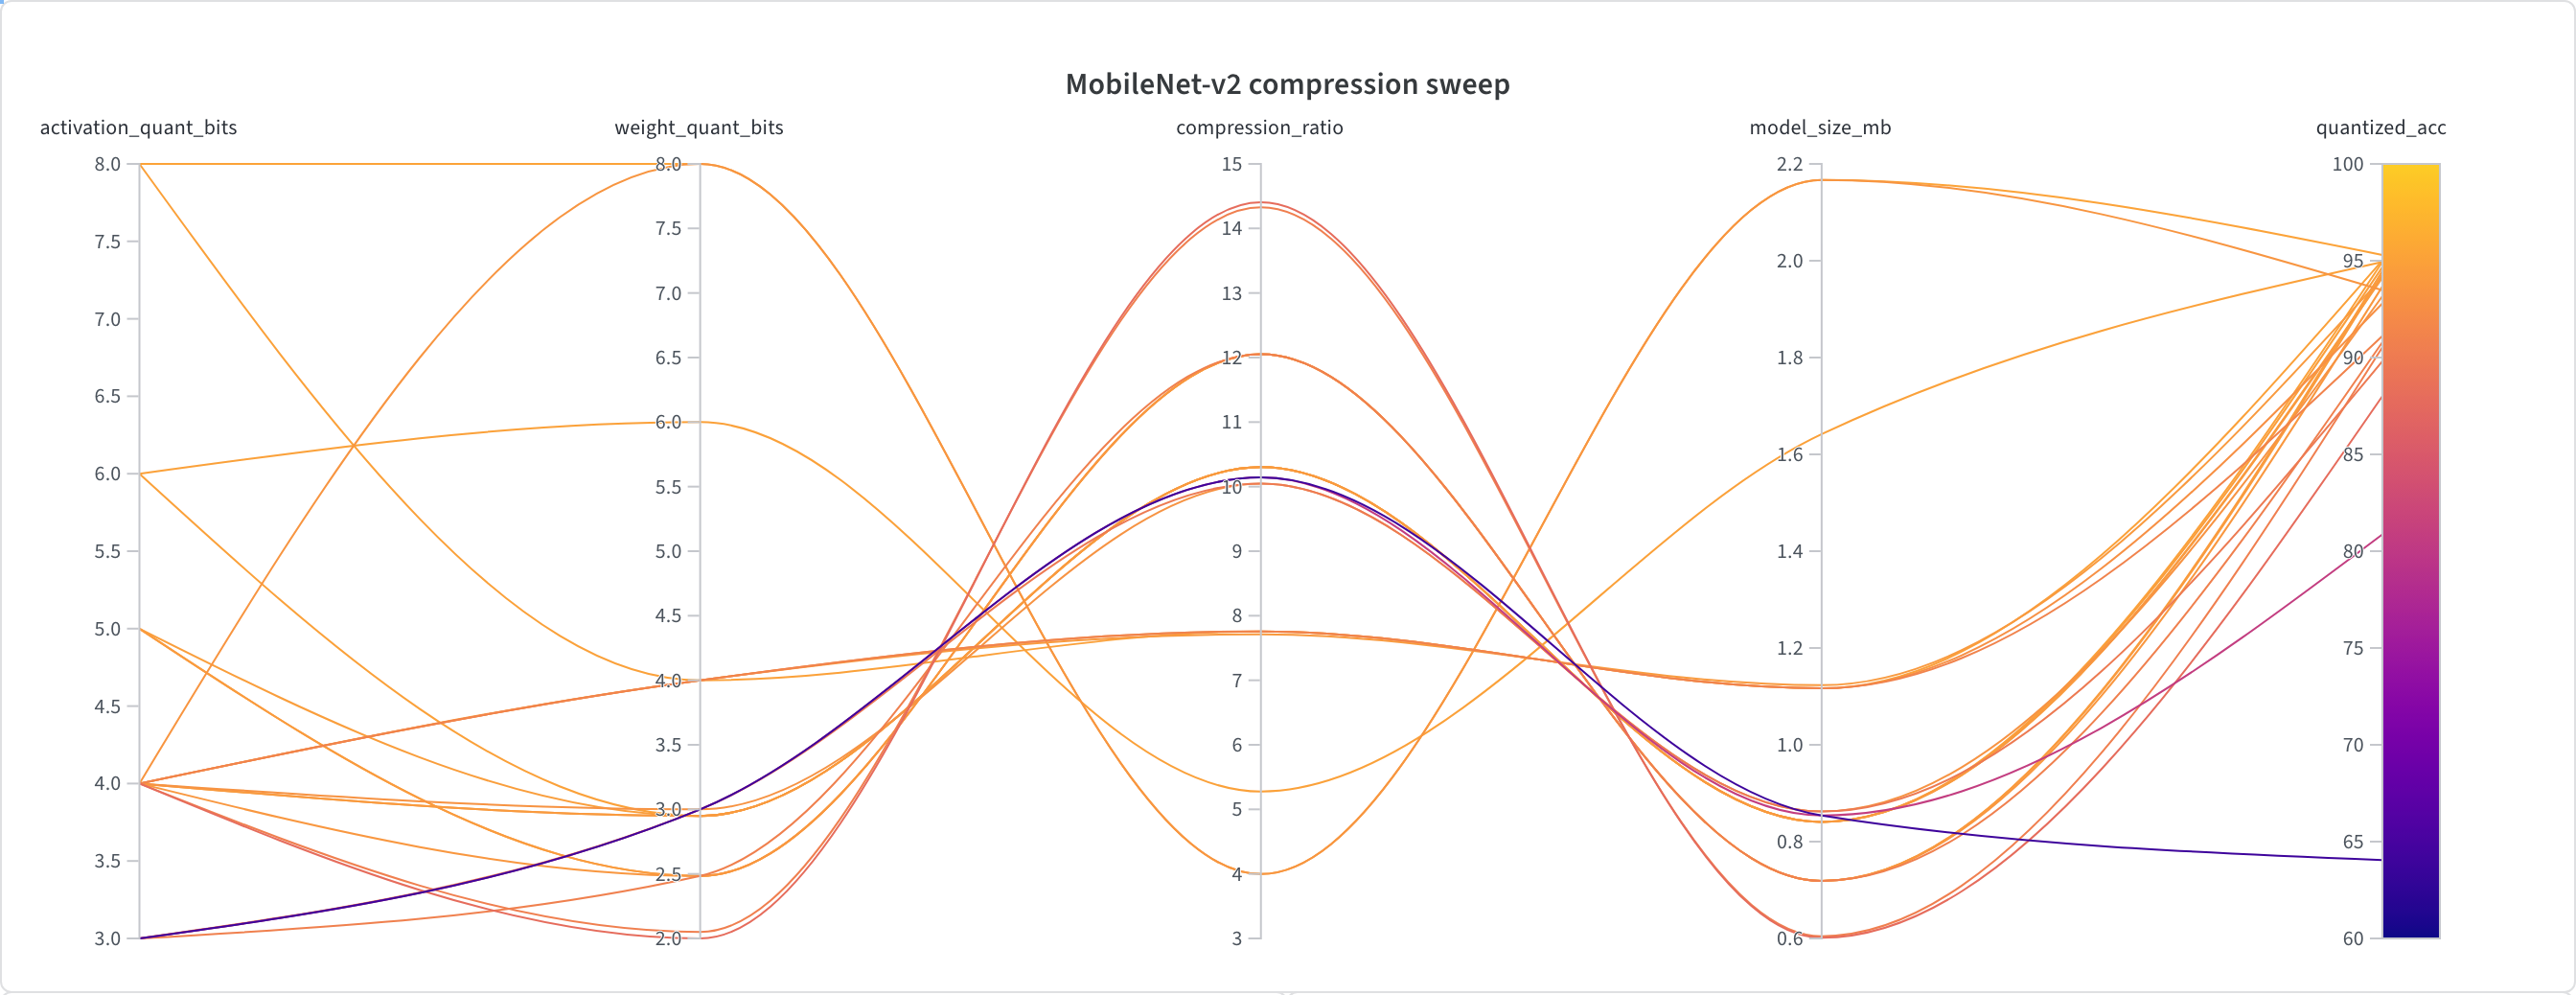
\includegraphics[width=\linewidth]{figures/wandb/parallel_coordinates.png}}{\fbox{W\&B chart pending}}
\caption{W\&B parallel-coordinates chart of the \NumRuns{} compression runs (rendered by W\&B from the logged runs): activation bits, average weight bits, model compression ratio, model size in MB and test accuracy of the compressed model.}
\label{fig:parallel}
\end{figure}

\begin{figure}[H]
\centering
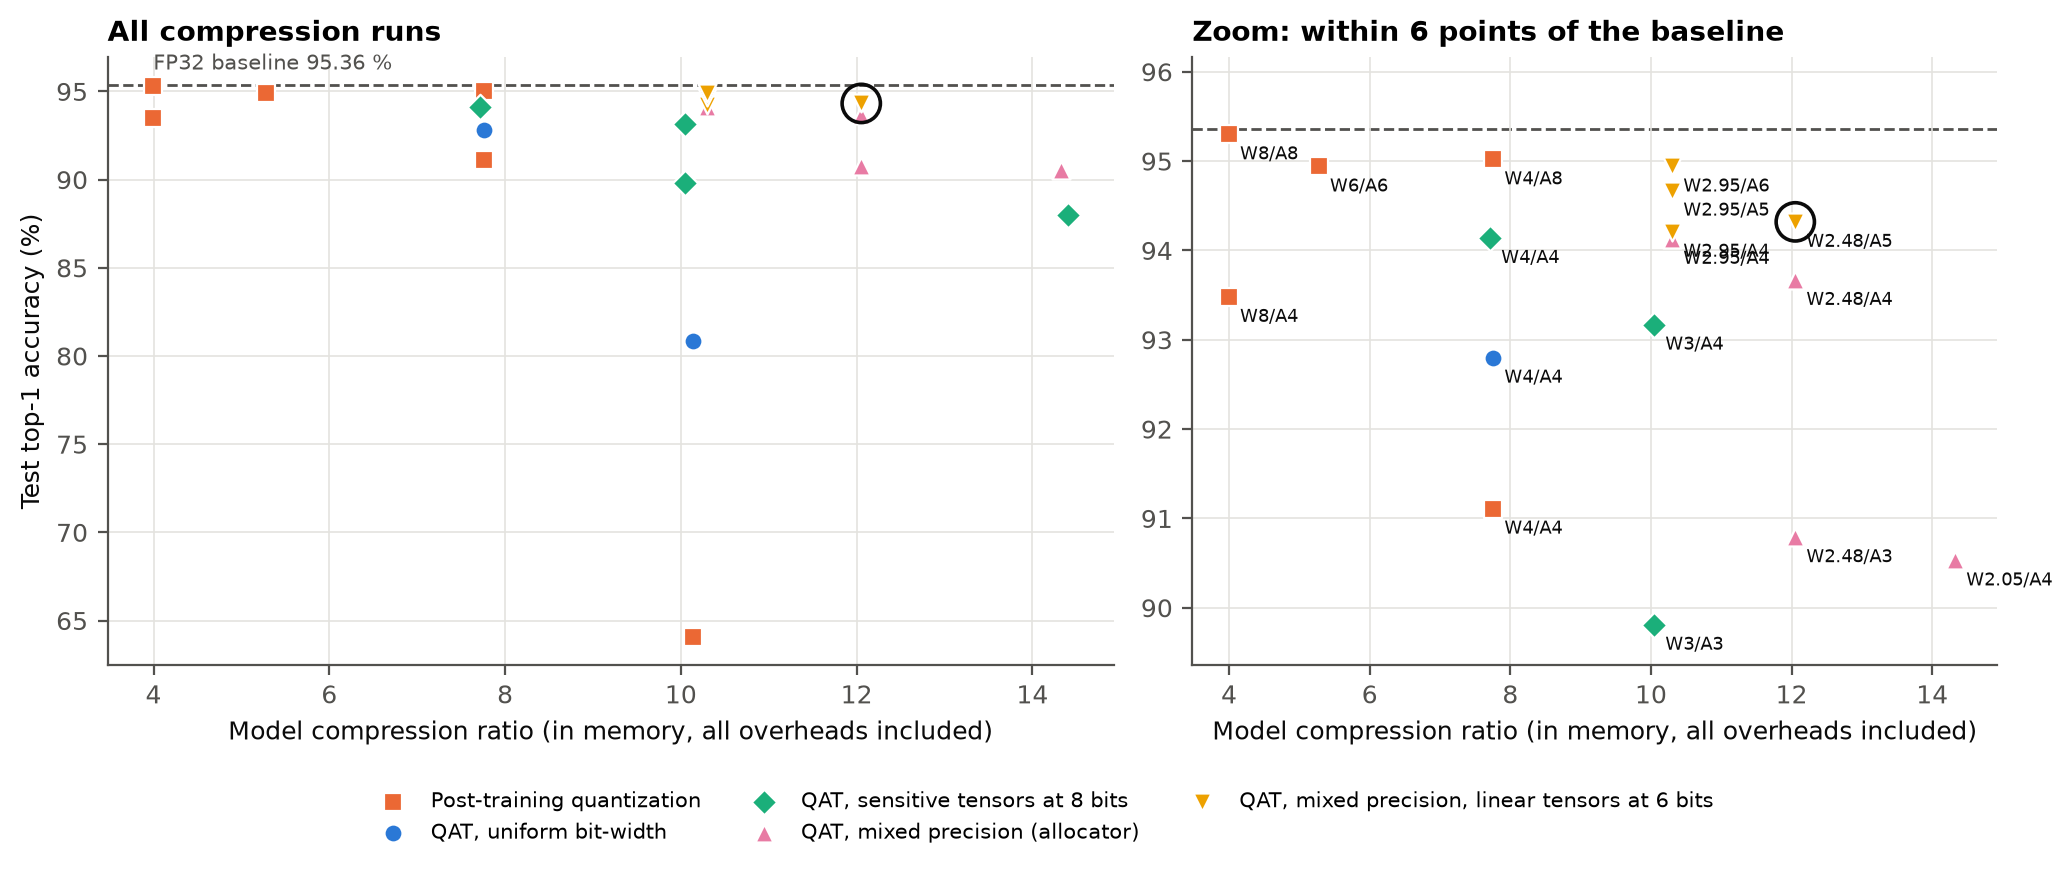
\includegraphics[width=\linewidth]{figures/tradeoff.png}
\caption{Test accuracy against model compression ratio for all runs. The dashed line is the FP32 baseline; the circled point is the final model.}
\label{fig:tradeoff}
\end{figure}

\SweepText

%=====================================================================
\section*{Question 4: Compression analysis}

All numbers in this section are for the final model \texttt{\BestName}.

\subsection*{(a) Compression ratio of the weights}

\WeightText

\subsection*{(b) Compression ratio of the activations}

\ActText

\begin{table}[H]
\centering
\small
\begin{tabular}{lrrrrr}
\toprule
Activation tensors & Tensors & Elements & Bits & FP32 bytes & Compressed bytes \\
\midrule
Input image (uint8 pixels) & 1 & 3,072 & 8 & 12,288 & 3,072 \\
ReLU6 feature maps (stem, expand, depthwise, head) & 35 & 1,502,208 & 8 & 6,008,832 & 1,502,208 \\
Linear bottleneck outputs and residual sums & 27 & 208,384 & 8 & 833,536 & 208,384 \\
Pooled feature vector & 1 & 1,280 & 8 & 5,120 & 1,280 \\
Logits & 1 & 10 & 32 & 40 & 40 \\
\midrule
Total (one image) & 65 & 1,714,954 & 8.00 (avg) & 6,859,816 & 1,714,984 \\
\bottomrule
\end{tabular}

\caption{Activation tensors of one forward pass of one image, by type.}
\label{tab:acts}
\end{table}

\begin{figure}[H]
\centering
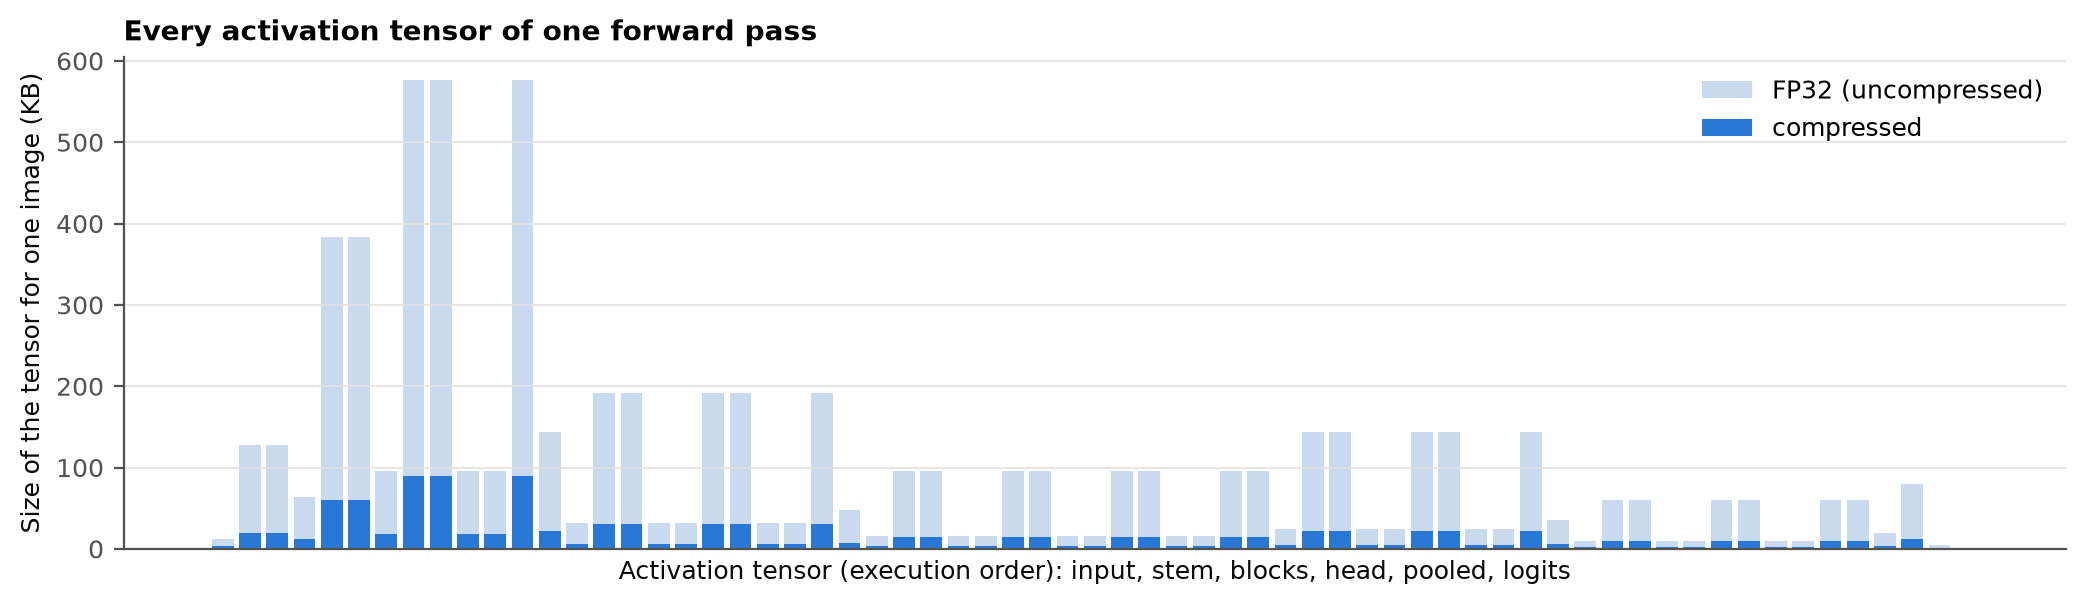
\includegraphics[width=\linewidth]{figures/activation_memory.png}
\caption{Size of every activation tensor for one image, uncompressed and compressed.}
\label{fig:acts}
\end{figure}

\subsection*{(v) Final approximated model size after compression}

\FinalSizeText

%=====================================================================
\section*{Question 5: Reproducibility and repository}

\textbf{(a) Code structure.} Training, evaluation and compression are separate:
\begin{center}
\small
\begin{tabular}{ll}
\toprule
File & Responsibility \\
\midrule
\texttt{mbv2/model.py}, \texttt{data.py}, \texttt{engine.py} & MobileNet-v2, CIFAR-10 pipeline, train / evaluate loops \\
\texttt{train.py} & baseline training (resumable) \\
\texttt{compress.py} & one compression run: calibration, PTQ or QAT, export, measurement \\
\texttt{test.py} & evaluation of the baseline and of a compressed model (template interface) \\
\texttt{run\_sweep.py} & the sweep of Question 3 \\
\texttt{compressor/quantizers.py} & learned-step uniform quantizer, hand-written gradients \\
\texttt{compressor/qmodel.py} & MobileNet-v2 with quantizers (training-time view) \\
\texttt{compressor/sensitivity.py} & per-layer sensitivity and mixed-precision bit allocation \\
\texttt{compressor/packing.py}, \texttt{packed.py} & bit-packing; the packed in-memory model and its export \\
\texttt{compressor/size.py}, \texttt{tracer.py} & model-size and activation-memory accounting \\
\texttt{tests/test\_compression.py} & 44 unit tests of all of the above \\
\texttt{scripts/} & figures, tables, failure analysis, W\&B report \\
\bottomrule
\end{tabular}
\end{center}

\textbf{(b) README.} The README gives the exact commands, the environment (macOS, Apple M1 Pro, Python 3.14.3, torch 2.14.1, torchvision 0.29.1, wandb 0.31.0; all pinned in \texttt{requirements.txt}) and the seed configuration (seed 42 for Python, NumPy, PyTorch, shuffling, augmentation and calibration subsets).

\textbf{(c) Repository:} \repo. It contains the trained baseline (\texttt{checkpoints/baseline.pt}) and the final compressed model (\texttt{checkpoints/compressed/best.pt}). The main commands are
\begin{Verbatim}[frame=single,fontsize=\small]
python train.py                                      # baseline (Question 1)
python test.py --weight_quant_bits 8 --activation_quant_bits 8   # template command (PTQ)
python run_sweep.py                                  # all compression runs (Question 3)
python test.py --checkpoint checkpoints/compressed/best.pt       # final compressed model
python -m pytest tests -q                            # unit tests
\end{Verbatim}

\end{document}
